\documentclass[a4paper,10pt]{scrartcl}

\usepackage[ngerman]{babel}
\usepackage[utf8]{inputenc}
\usepackage[T1]{fontenc}
\usepackage[babel,german=quotes]{csquotes}
\usepackage{hyperref}
\usepackage{geometry}
\usepackage{graphicx}
\usepackage{enumitem}
\usepackage{multicol}

\setlength\parindent{0pt}
\setitemize{itemsep=0pt}


\geometry{
	a4paper,
	left=20mm,
	top=20mm,
	bottom=15mm,
	footskip=5mm
}


\title{Pflichtenheft für das Thema \glqq\textit{Klick-Tool}\grqq}
\subtitle{Betreuer: \textit{Prof. Dr. Andreas Nüchter}}
\author{\textit{Tom Lerzer, Fabia Frank, Luis Ángel Álvarez Gil}}
\date{\textit{SS2026}}

\begin{document}

\maketitle



\section{Zielbestimmung}

\subsection{Muss-Kriterien}

\begin{itemize}
    \item Laden von Bilddaten in jpg und png Format
    \item Internes Erstellen von png-Dateien bei Eingabe von 3DTK-spezifischen 3D-Dateiformaten
    \item Implementieren eines GUI zur erleichterten Ausführung der implementierten Funktionalitäten
    \item Platzieren von maximal zwei der geladenen Bilder nebeneinander
    \item Zoom-Funktion für 20-fachen Zoom jedes geladenen Bildes
    \item Anwählen einzelner Koordinaten in einem Bild mit Subpixelgenauigkeit von mindestens 0,1 Pixel
    \item Anwählen korrespondierender Koordinaten in zwei Bildern mit Subpixelgenauigkeit von mindestens 0,1 Pixel
    \item Visualisierung gewählter Koordinaten
    \item Visualisierung der Korrespondenz gewählter Koordinaten
    \item Ausgabe gewählter 2D-Koordinaten in Form $x_1, y_1, \backslash n, ..., x_n, y_n, \backslash n$ für einfache bzw. $x_{1.1}, y_{1.1}, y_{1.2}, y_{1.2}, \backslash n ,$ $ ..., x_{n.1}, y_{n.1}, x{n.2}, y_{n.2},  \backslash n$ in txt-Dateiformat
    \item Integration der implementierten Funktionalitäten in 3DTK-Toolkit 
    \item Implementieren von Kommandozeilenparametern sowie deren Beschreibungen für das Aufrufen der implementierten Funktionalitäten
    \item Erstellen eines Entwicklerhandbuchs für die implementierten Funktionalitäten
    \item Erstellen eines Benutzerhandbuchs für die implementierten Funktionalitäten
\end{itemize}

\subsubsection{Halbzeit-Ziele}
\begin{itemize}
\item Laden von Bilddaten in jpg und png Format
\item Internes Erstellen von png-Dateien bei Eingabe von 3DTK-spezifischen 3D-Dateiformaten
\item Implementieren eines GUI zur erleichterten Ausführung der implementierten Funktionalitäten
\item Platzieren von maximal zwei der geladenen Bilder nebeneinander
\item Zoom-Funktion für 20-fachen Zoom jedes geladenen Bildes
\item Anwählen einzelner Koordinaten in einem Bild mit Subpixelgenauigkeit von mindestens 0,1 Pixel
\item Anwählen korrespondierender Koordinaten in zwei Bildern mit Subpixelgenauigkeit von mindestens 0,1 Pixel
    
\end{itemize}
\newpage

\subsubsection{Zuständigkeiten}
Aufgrund des gewählten agilen Entwicklungsansatzes mit pair-programming werden keine festen Zuständigkeiten festgelegt. 

\subsection{Kann-Kriterien}

\begin{itemize}
    \item Automatische Wahl der optimalen Anordnung der Bilder (nebeneinander oder übereinander) aufgrund Bildgröße und Bildschirmauflösung
    \item Ausblenden einzelner Korrespondenzlinien zwischen Punkten
    \item Anzeige Koordinaten der gewählten Punkte
    \item Undo-Funktion für ausgewählte Punkte
    \item Verbesserte Pixeldarstellung bei Zoom
\end{itemize}

\subsection{Abgrenzungskriterien}

\begin{itemize}
    \item Anwahl korrespondierender Punkte wird ausschließlich manuell durchgeführt
    \item Die Funktionalität für die Umwandlung von 3D-Formaten ist bereits vorhanden und muss in das Projekt integriert werden.
\end{itemize}


\section{Einsatz}

\subsection{Anwendungsbereiche}
\begin{itemize}
	\item Bildverarbeitung
	\item Robotik
	\item Photogrammetrie
\end{itemize}


\subsection{Zielgruppe}

Das Projekt soll durch Studierende und Lehrende der Universität Würzburg im Rahmen der Robotik-Forschung, der Bildverarbeitung sowie allgemein im Bereich Informatik zum Einsatz gebracht werden. Für weitere interessierte Personen ist das Projekt auf GitHub zugänglich.


\section{Umgebung}

\subsection{Software}

\begin{itemize} 
\item Programmiersprache: C++ Version 17 \url{https://isocpp.org/} 
\item Laden von Bilddateien: stb\_image.h Version 2.30 \url{https://github.com/nothings/stb/blob/master/stb_image.h} 
\item Benutzungsoberfläche: Dear ImGUI Version 1.90 \url{https://github.com/ocornut/imgui} 
\item 3D-Framework: 3DTK \url{https://github.com/JMUWRobotics/3DTK} 
\item Editor: Visual Studio Code Version 1.119 \url{https://code.visualstudio.com/} 
\item Compiler: g++ Version 15.2 \url{https://gcc.gnu.org/} 
\item Build-System: CMake Version 3.15 \url{https://cmake.org/} 
\item Versionsverwaltung: git Version 2.51 \url{https://git-scm.com/} 
\item Fensterverwaltung: GLFW Version 3.4 \url{https://www.glfw.org/} 
\item Grafik-API: OpenGL Version 4.6 \url{https://www.opengl.org/} \end{itemize}

\subsection{Hardware}

Die Hardware muss alle Anforderungen der im vorherigen Punkt genannten Software erfüllen.

\section{Funktionalität}

\begin{itemize}
	\item Nutzer starten das Programm via Terminal. Beim Start des Programms werden keine, ein oder zwei Parameter in den unter \hyperref[daten]{Daten} angegebenen Formaten eingegeben. Beim Start ohne Parameter öffnet sich das GUI ohne geladene Bilder. Diese können nachträglich in der Load-Section geladen werden. 
	\item Optional kann ein Speicherort für die Ausgabe der Koordinaten und der konvertierten 3D-Bilder angegeben werden
	\item Auf dem angezeigten Bild bzw. den angezeigten Bildern kann vor der weiteren Bearbeitung bis zu 20-Mal hineingezoomt werden
	\item Die Nutzer wählen beliebig viele einzelne oder korrespondierende Punkte aus
	\item Das Programm zeigt die angewählten Punkte und deren Korrespondenzen im GUI an
	\item Durch Anwählen des Buttons ''Speichern \& Beenden'' initiieren Nutzer die Speicherung der gewählten Punkte in txt-Format am festgelegten oder default-Speicherort 
\end{itemize}


\section{Daten}
\label{daten}
\begin{itemize}
	\item \textbf{Eingabe:} Dateien im png oder jpg-Format sowie 3DTK-spezifische Formate, die durch Anwendung der \textit{scan\_to\_panorama}-Funktion in anzeigbare png-Dateien umgewandelt werden
	\item \textbf{Ausgabe:} txt-Datei mit Koordinaten in Form $x_1, y_1, \backslash n, ..., x_n, y_n, \backslash n$ für einfache bzw. $x_{1.1}, y_{1.1}, y_{1.2}, y_{1.2}, \backslash n ,$ $ ..., x_{n.1}, y_{n.1}, x{n.2}, y_{n.2},  \backslash n$ für korrespondierende Punkte
	\item \textbf{3DTK-spezifische Formate:} uos, uos\_map, uos\_rgb, uos\_frames, uos\_map\_frames
	
\end{itemize}



\section{Leistungen}

Das Laden der Bilddateien, die Umwandlung der 3DTK-spezifischen Datenformate, die Zoom-Funktionalität sowie Auswahl und Ausgabe der gewählten Koordinaten soll weitestgehend performant sein und so in einer angemessenen Zeit geschehen.


\section{Benutzungsoberfläche}
\graphicspath{/home/fabia/Schreibtisch/SWP/3DTK/src/slam6d/fbr/new_click_tool/docs/Pflichtenheft}
\begin{minipage}{0.5\textwidth}
	\begin{enumerate}
		\item Hauptfenster: Anzeige eines oder zweier Bilder sowie Zoom-Funktion zur Auswahl von Punkten bzw. Punktkorrespondenzen
		\item Steuerungsfenster: Hilfe-Funktion, Laden von Bildern, Einstellungen bzgl. Bildmodus, Auswahlmodus, Ausgabeort, Undo-Funktion sowie Speichern und Beenden
		\item Load-Section: Setzen des Output-Directories und Laden von ein oder zwei Bildern bzw. Scans
		\item Auswahl-/Anzeigemodus, Sicht zentrieren
		\item Anzeige Anzahl Punkte, Speicherort, Undo-Funktion, Speichern und Beenden
	\end{enumerate}
\end{minipage}
\begin{minipage}{0.6\textwidth}
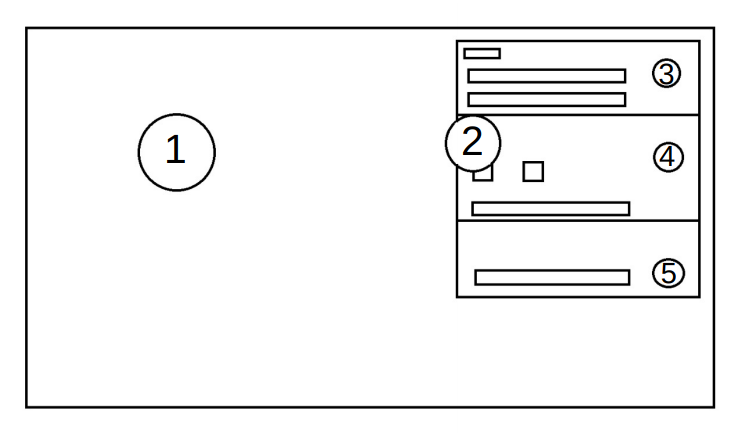
\includegraphics[width=\linewidth]{GuiSkizze.png}


\end{minipage}



\section{Qualitätsziele}

Der Code soll gut kommentiert und klar strukturiert sein, sodass sich neue Entwicklerinnen und Entwickler gut in dem Projekt zurechtfinden und es leicht erweitern und ändern können. Um dies zu erleichtern, wird außerdem ein Developerhandbuch erstellt.\\
Das Ergebnis des Projekts soll eine hohe Benutzerfreundlichkeit haben und für Anwenderinnen und Anwender wird zusätzlich ein Benutzerhandbuch bereitgestellt.

\end{document}